% ****** Start of file apssamp.tex ******
%
%   This file is part of the APS files in the REVTeX 4.2 distribution.
%   Version 4.2a of REVTeX, December 2014
%
%   Copyright (c) 2014 The American Physical Society.
%
%   See the REVTeX 4 README file for restrictions and more information.
%
% TeX'ing this file requires that you have AMS-LaTeX 2.0 installed
% as well as the rest of the prerequisites for REVTeX 4.2
%
% See the REVTeX 4 README file
% It also requires running BibTeX. The commands are as follows:
%
%  1)  latex apssamp.tex
%  2)  bibtex apssamp
%  3)  latex apssamp.tex
%  4)  latex apssamp.tex
%
\documentclass[%
 reprint,
%superscriptaddress,
%groupedaddress,
%unsortedaddress,
%runinaddress,
%frontmatterverbose, 
%preprint,
%preprintnumbers,
%nofootinbib,
%nobibnotes,
%bibnotes,
 amsmath,amssymb,
 aps,
 pra,
%prb,
%rmp,
%prstab,
%prstper,
%floatfix,
]{revtex4-2}
\usepackage[spanish,es-nodecimaldot]{babel}
\usepackage{color,soul}
\usepackage{physics}
\usepackage{minted}
\usepackage{graphicx}% Include figure files
%\usepackage{svg}
\usepackage{dcolumn}% Align table columns on decimal point
\usepackage{bm}% bold math
\usepackage{hyperref}% add hypertext capabilities
\definecolor{linkcolour}{rgb}{0,0.2,0.6} % Link color
\hypersetup{colorlinks,citecolor=linkcolour,breaklinks,urlcolor=linkcolour,linkcolor=linkcolour}
\usepackage{color,soul}
\usepackage{soulutf8}
\usepackage{mathrsfs}
\usepackage{wrapfig}
%\usepackage[mathlines]{lineno}% Enable numbering of text and display math
%\linenumbers\relax % Commence numbering lines

%\usepackage[showframe,%Uncomment any one of the following lines to test 
%%scale=0.7, marginratio={1:1, 2:3}, ignoreall,% default settings
%%text={7in,10in},centering,
%%margin=1.5in,
%%total={6.5in,8.75in}, top=1.2in, left=0.9in, includefoot,
%%height=10in,a5paper,hmargin={3cm,0.8in},
%]{geometry}

\begin{document}

\preprint{APS/123-QED}

\title{Modelo de Ising:\texorpdfstring{\\}{ }Apreciaciones Generales y Algoritmo Metrópolis.}% Force line breaks with \\

\author{Juan Esteban Aristizabal Zuluaga}
\affiliation{Instituto de Física, Universidad de Antioquia.}%Lines break automatically or can be forced with \\

\date{\today}% It is always \today, today,
             %  but any date may be explicitly specified

\begin{abstract}

\begin{description}
\item[Palabras clave] 	.
\end{description}
\end{abstract}

%\keywords{Suggested keywords}%Use showkeys class option if keyword
                              %display desired
\maketitle

%\tableofcontents
\onecolumngrid


	
\section{Introducción\label{sec:intro}}

\section{Consideraciones teóricas\label{sec:teoria}}

	\subsection{Hamiltoniano del sistema\label{subsec:teoria-hamiltoniano}}
	
	\subsection{Microestados y contribuciones a la función partición\label{subsec:teoria-contribuciones-Z}}
	
		\begin{figure}[!ht]
			\centering
			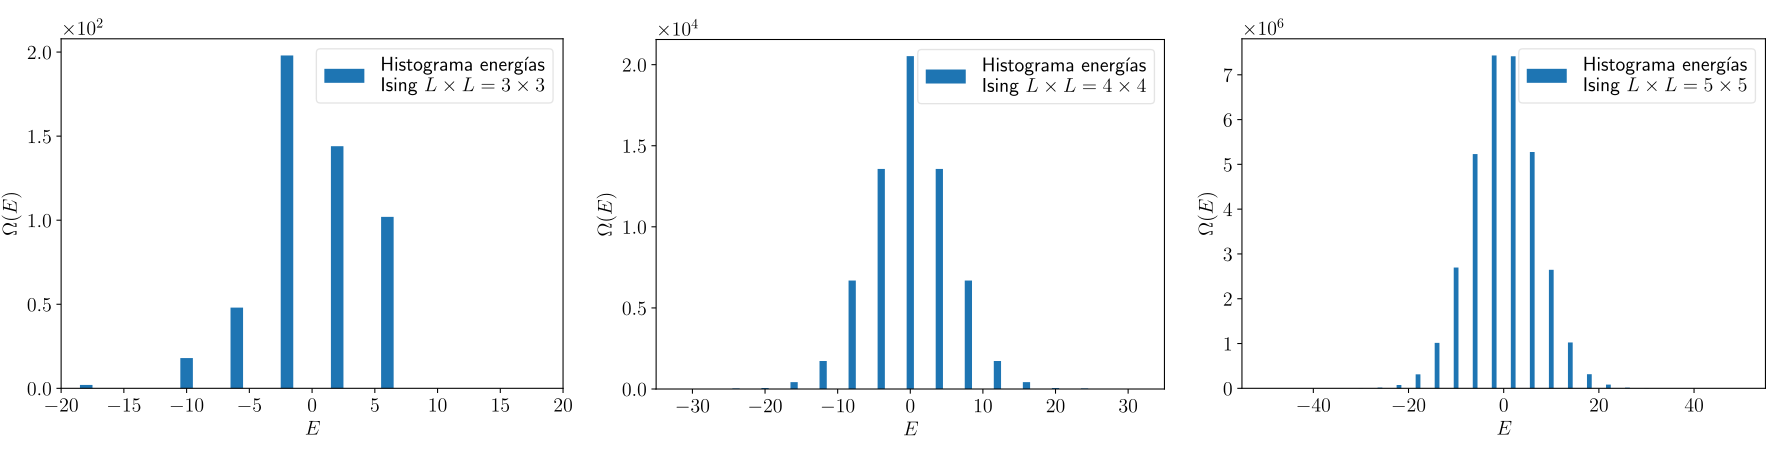
\includegraphics[width=\linewidth]{{{figures/ising-energy-plots-L_3_4_5}}}
			\caption{}
			\label{fig:energy-omegas-3x3-4x4-5x5}
		\end{figure}

		\begin{figure}[!ht]
			\centering
			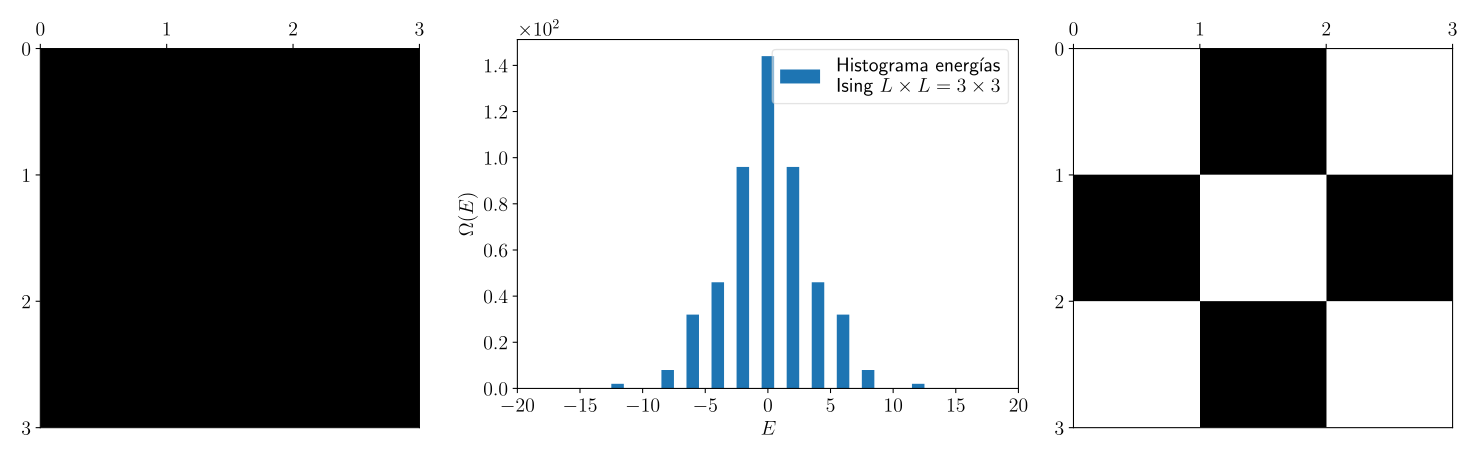
\includegraphics[width=0.9\linewidth]{{{figures/ising-odd_asymmetry-L_3}}}
			\caption{}
			\label{fig:energy-asymmetry-fbc-3x3}
		\end{figure}

	\subsection{Equivalencia entre ensambles microcanónico y macrocanónico\label{subsec:teoria-equivalencia-micro}}
	
		\begin{figure}[!ht]
			\centering
			\includegraphics[width=0.4\linewidth]{{{figures/ising-Z_approx-plot-L_3_4_5}}}
			\caption{}
			\label{fig:micro-macro-equivalence}
		\end{figure}

	\subsection{Teorema de fluctuación-disipación y calor específico\label{subsec:teoria-calor-especifico}}

		\begin{figure}[!ht]
			\centering
			\includegraphics[width=0.4\linewidth]{{{figures/ising-specific_heat-plot-L_2_3_4_5}}}
			\caption{}
			\label{fig:specific-heat}
		\end{figure}
	

\section{Modelo de Ising y Algoritmo Metrópolis\label{sec:resultados}}
	\subsection{El algoritmo\label{subsec:metropolis-algoritmo}}
		\inputminted[linenos,breaklines]{python}{ising2d-metropolis-z-retazo.py}
	\subsection{Termalización del sistema usando el algoritmo\label{subsec:metropolis-termalizacion}}

	\begin{figure}[!ht]
		\centering
		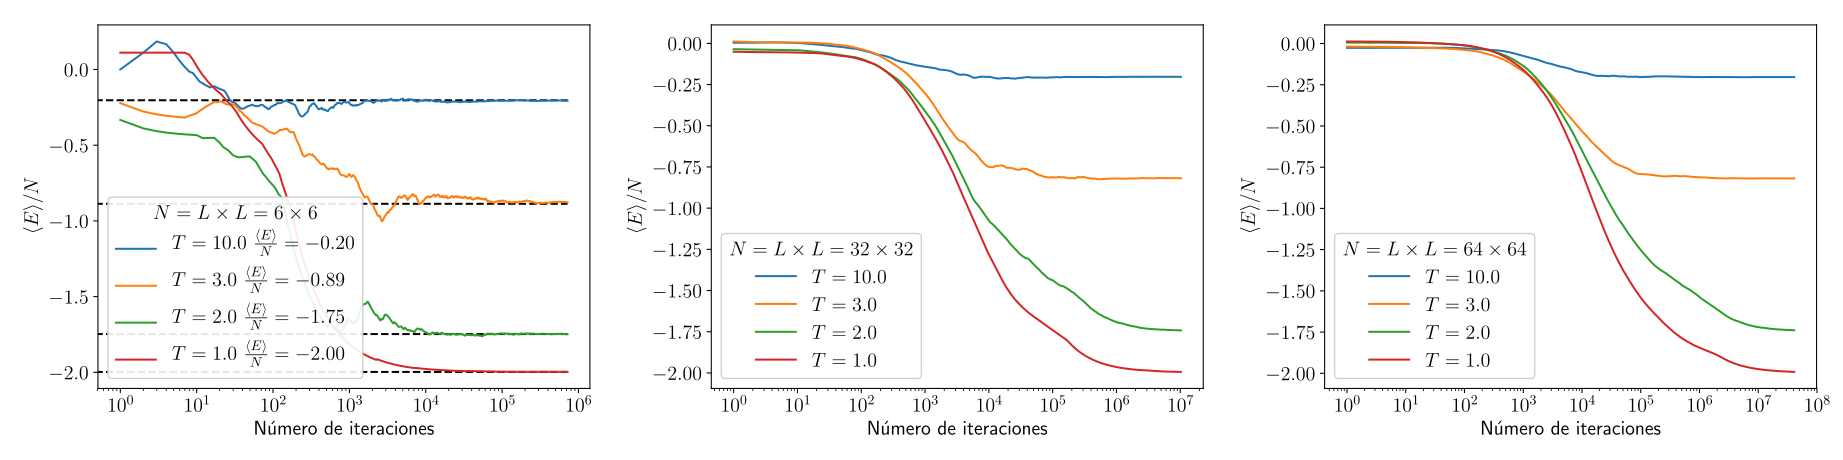
\includegraphics[width=\linewidth]{{{figures/ising-metropolis-thermalization-plot-L_6_32_64-T_10.0_3.0_2.0_1.0}}}
		\caption{}
		\label{fig:thermalization-energy}
	\end{figure}
	
	\begin{figure}[!ht]
		\centering
		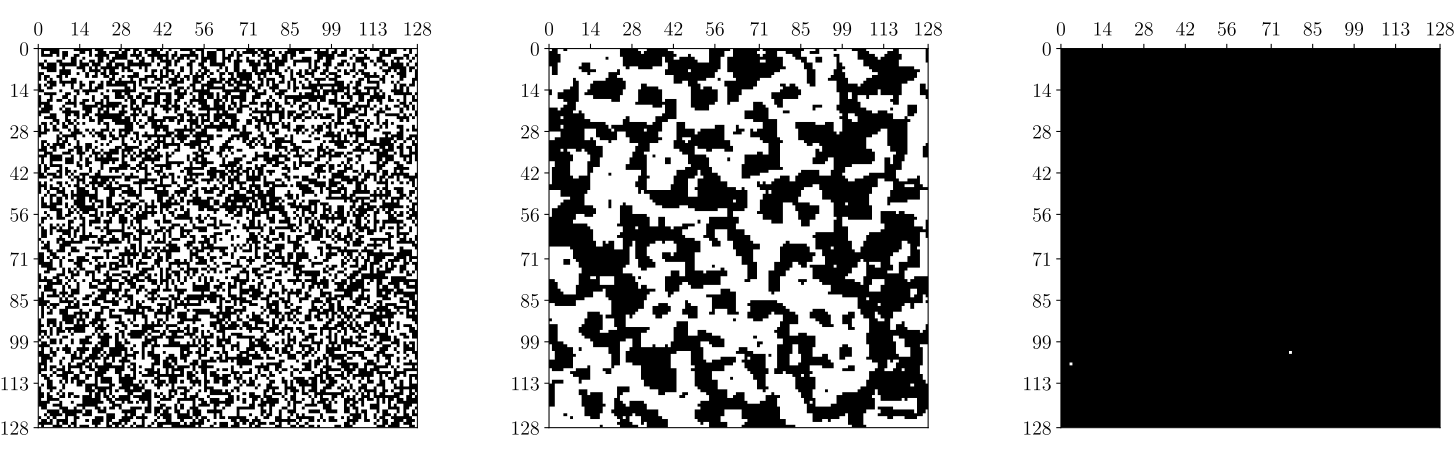
\includegraphics[width=\linewidth]{{{figures/ising-metropolis-config-plot-L_128-thermalization}}}
		\caption{}
		\label{fig:thermalization-configs}
	\end{figure}

	\subsection{Microestados finales y temperatura crítica\label{subsec:metropolis-microestados-temp-critica}}

	\begin{figure}[!ht]
		\centering
		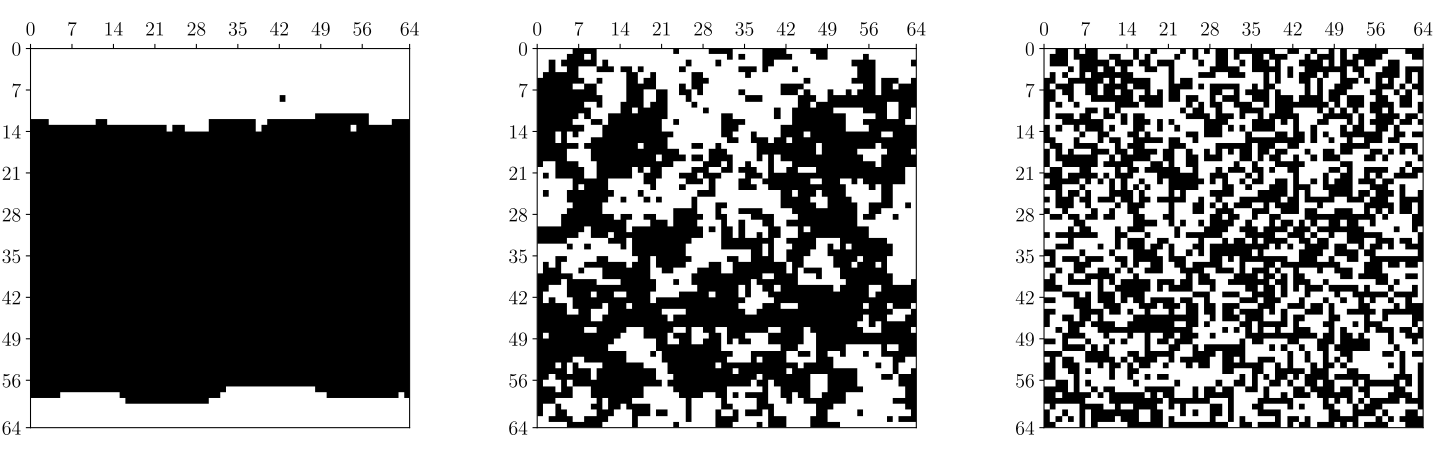
\includegraphics[width=\linewidth]{{{figures/ising-metropolis-config-plot-L_64-temp_1.000_2.500_10.000-typical}}}
		\caption{}
		\label{fig:final-thermalized-microstates-different-temperatures}
	\end{figure}

	\begin{figure}[!ht]
		\centering
		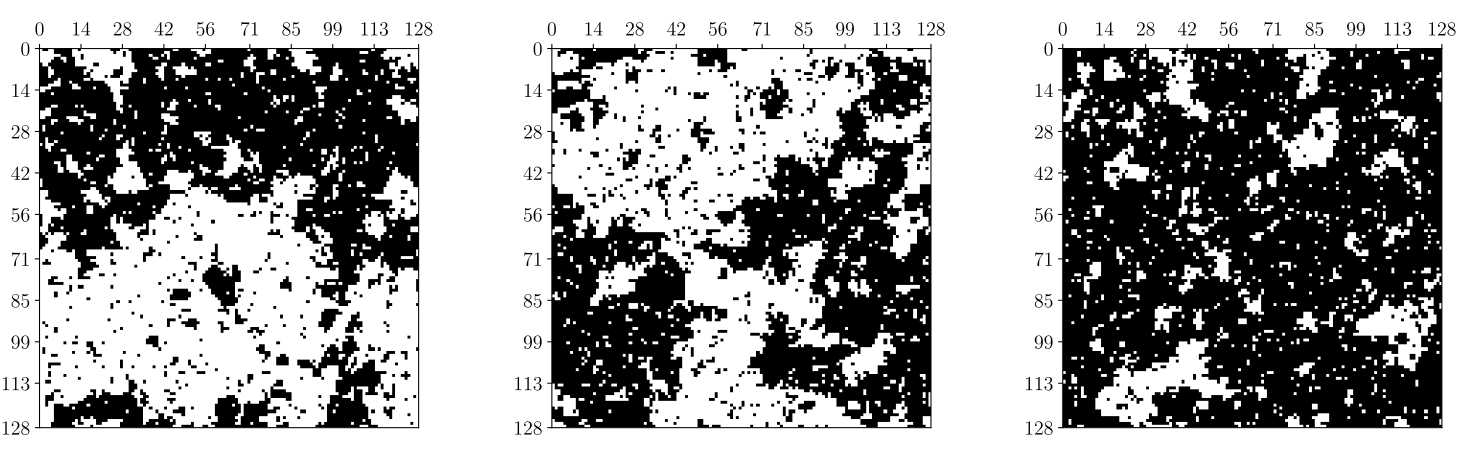
\includegraphics[width=\linewidth]{{{figures/ising-metropolis-config-plot-L_128-temp_2.270-critical-temp}}}
		\caption{}
		\label{fig:final-critical-temp-128x128}
	\end{figure}

	\subsection{Calor específico\label{subsec:metropolis-cv}}

	\begin{figure}[!ht]
		\centering
		\includegraphics[width=0.4\linewidth]{{{figures/ising-metropolis-specific_heat-plot-L_2_3_4_5_8_16_32_64-N_steps_factor_80000}}}
		\caption{}
		\label{fig:metropolis-cv}
	\end{figure}



\section{Conclusión\label{sec:conclusion}}



Las implementaciones de los algoritmos usados en este trabajo son suficientemente generales y se podrían adaptar con cierta facilidad a otros sistemas de interés que sean objeto de estudio.

\section*{Agradecimientos}
Agradezco a mis compañeros de clase con los que tuve discusiones que ayudaron en la implementación del algoritmo y en las conclusiones presentadas.

\nocite{*}

\bibliography{5-Semestre_X_2020_I-Fisica_Estadistica_Avanzada-Tarea_3}% Produces the bibliography via BibTeX.



\newpage


\appendix

\begin{widetext}

\section{Código 1: Matrix Squaring\label{appx:codigo_matrix_squaring}}

A continuación se muestra el código . Éste código está disponible en \href{https://github.com/jearistiz/Statistical-Physics-Projects/blob/master/2/matrix_squaring.py}{este link}

%\inputminted[linenos,breaklines]{python}{code_1.py}

\section{Código 2: Naive Path Integral Montecarlo Sampling\label{appx:codigo-path-int}}

A continuación se muestra el código que está disponible en \href{https://github.com/jearistiz/Statistical-Physics-Projects/blob/master/2/path_integral_naive_sampling.py}{este link}.

%\inputminted[linenos,breaklines]{python}{code_2.py}

\end{widetext}


\end{document}
%
% ****** End of file apssamp.tex ******
